% Asset ID: A21FunctionsAndGraphsTIKZ-001
% Unit: A21: A2 1 Pure Mathematics
% Topic code: A21-AF
% Related LO IDs: A21-AF-LO006
% Related lesson section: The Graph of y = |x|
% Source: Chapter 2 Functions and Graphs lesson evidence, modulus graph section
% Purpose: Show the V-shaped graph of y = |x|.

\documentclass[tikz,border=8pt]{standalone}
\usepackage{amsmath}
\usetikzlibrary{arrows.meta}
\begin{document}
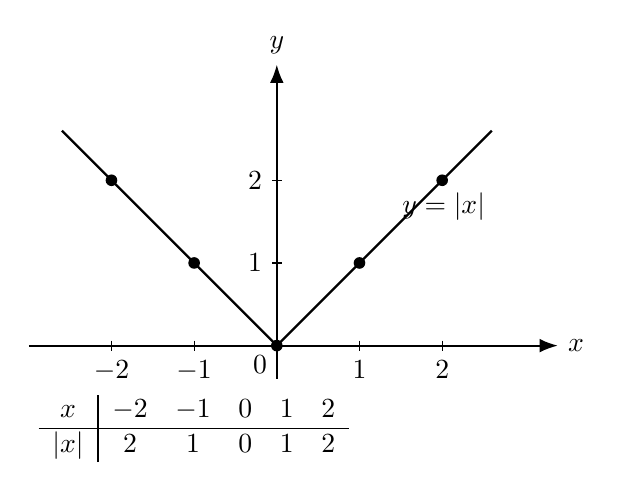
\begin{tikzpicture}[scale=1.05, >=Latex]
\draw[->, thick] (-3,0) -- (3.4,0) node[right] {$x$};
\draw[->, thick] (0,-0.4) -- (0,3.4) node[above] {$y$};
\foreach \x in {-2,-1,1,2} \draw (\x,0.06) -- (\x,-0.06) node[below] {$\x$};
\foreach \y in {1,2} \draw (0.06,\y) -- (-0.06,\y) node[left] {$\y$};
\node[below left] at (0,0) {$0$};
\draw[thick] (-2.6,2.6) -- (0,0) -- (2.6,2.6);
\foreach \x/\y in {-2/2,-1/1,0/0,1/1,2/2} {\fill (\x,\y) circle (2pt);}
\node[above right] at (1.4,1.4) {$y=|x|$};
\node[align=left, anchor=west] at (-3,-1.0) {$\begin{array}{c|ccccc}x & -2 & -1 & 0 & 1 & 2\\\hline |x| & 2 & 1 & 0 & 1 & 2\end{array}$};
\end{tikzpicture}
\end{document}
